\section{A tool for seed image analysis}
ImageJ allows the realisation of new plugins, e.g., dealing with specific problems in the image analysis field or computing new features in different contexts.
Among the state-of-the-art, different plugins already exist and can extract features from seeds images, even though they are general-purpose. One of them is \emph{Particles8} \cite{Landini}, created by Gabriel Landini in 2005, with the last update in 2010. It provides the extraction of morphological features from binary images. Consequently, it does not provide the extraction of textural and colour features.
To simplify the botanists' seed analysis procedures, we followed their indications, and we realised a brand new plugin exclusively with \emph{ImageJ} classes without using any external plugins and increasing its extensibility. The proposed tool allows the extraction and classification of features and can be used in many other application domains.

\subsection{A plugin for feature extraction from seeds image}
\label{seeds_analyser}
\emph{SeedsAnalyser} is the plugin for feature extraction proposed in this work and needs a minimal number of user interactions. It aims to identify and analyse multiple seeds represented in a digital image. The input is a single image acquired with a quasi-uniform blue background.
The plugin is also able to analyse all the images in a specific folder at the same time. Each image can present a blue background in a wide range of tones, varying from a very light blue to a very dark navy blue. After the acquisition, the image is preprocessed for the correct separation of the regions of interest, namely the single seeds. 
It is possible to isolate the Blue value of the RGB images to get pure masks as the dataset backgrounds are all in various shades of blue (see Figure \ref{Sardinia_Masks}), as indicated in our previous work \cite{Loddo20}. 
Creating a single seed dataset from the original database is possible thanks to different backgrounds of various blue shades. It allowed finding the best images to work on and making the binary masks to extract the single seeds just by an automatic thresholding procedure.
During the acquisition, the seeds were well spaced from each other. Therefore the bounding box of each region allowed the creation of a single seed image for analysis quickly.
From the \emph{Fabaceae} dataset, we selected the images containing the most numerous samples per species for 23 different species and nearly 2000 seeds.
We discarded some species due to the low sharpness and too small size of the seeds. Figures \ref{Sardinia_Masks} and \ref{Sardinia_Crops} show an original sample image with its derived binary mask and some seed images extracted from it, respectively. 
\begin{figure}[htbp]
	\centering
	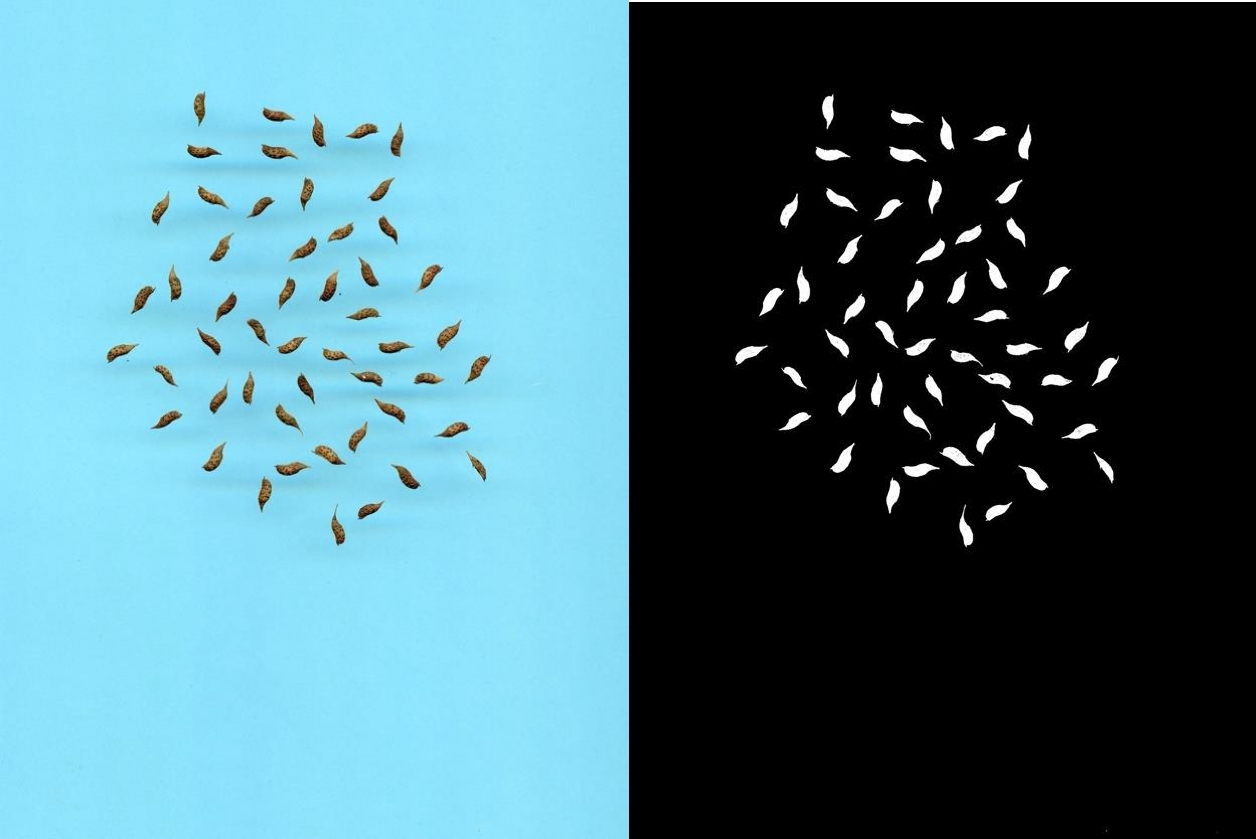
\includegraphics[scale=0.6]{SardiniaMasks.jpg}
	\caption{Example of an image from the \emph{Fabaceae} database and its derived binary mask.}
	\label{Sardinia_Masks}
\end{figure}

\begin{figure}[htbp]
	\centering
	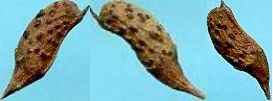
\includegraphics[scale=0.4]{Sardinia_crops.jpg}
	\caption{Some examples of seed images extracted from the image of Figure \ref{Sardinia_Masks} of the \emph{Fabaceae} database.}
	\label{Sardinia_Crops}
\end{figure}

Once the images have been preprocessed, i.e. segmented by automatic thresholding, and the unique image is ready to be analyzed, the plugin requires the selection of some key parameters. They improve the research and detection of the regions of interest, specifically the minimum and maximum area size, measured in square pixels and, if wanted, a specific circularity of the objects, by default ranging from 0 to 1.
Finally, the users can choose the features of interest from the "Feature" window, as shown in Figure \ref{fig:features_selection}.

\begin{figure}[htbp]
	\centering
	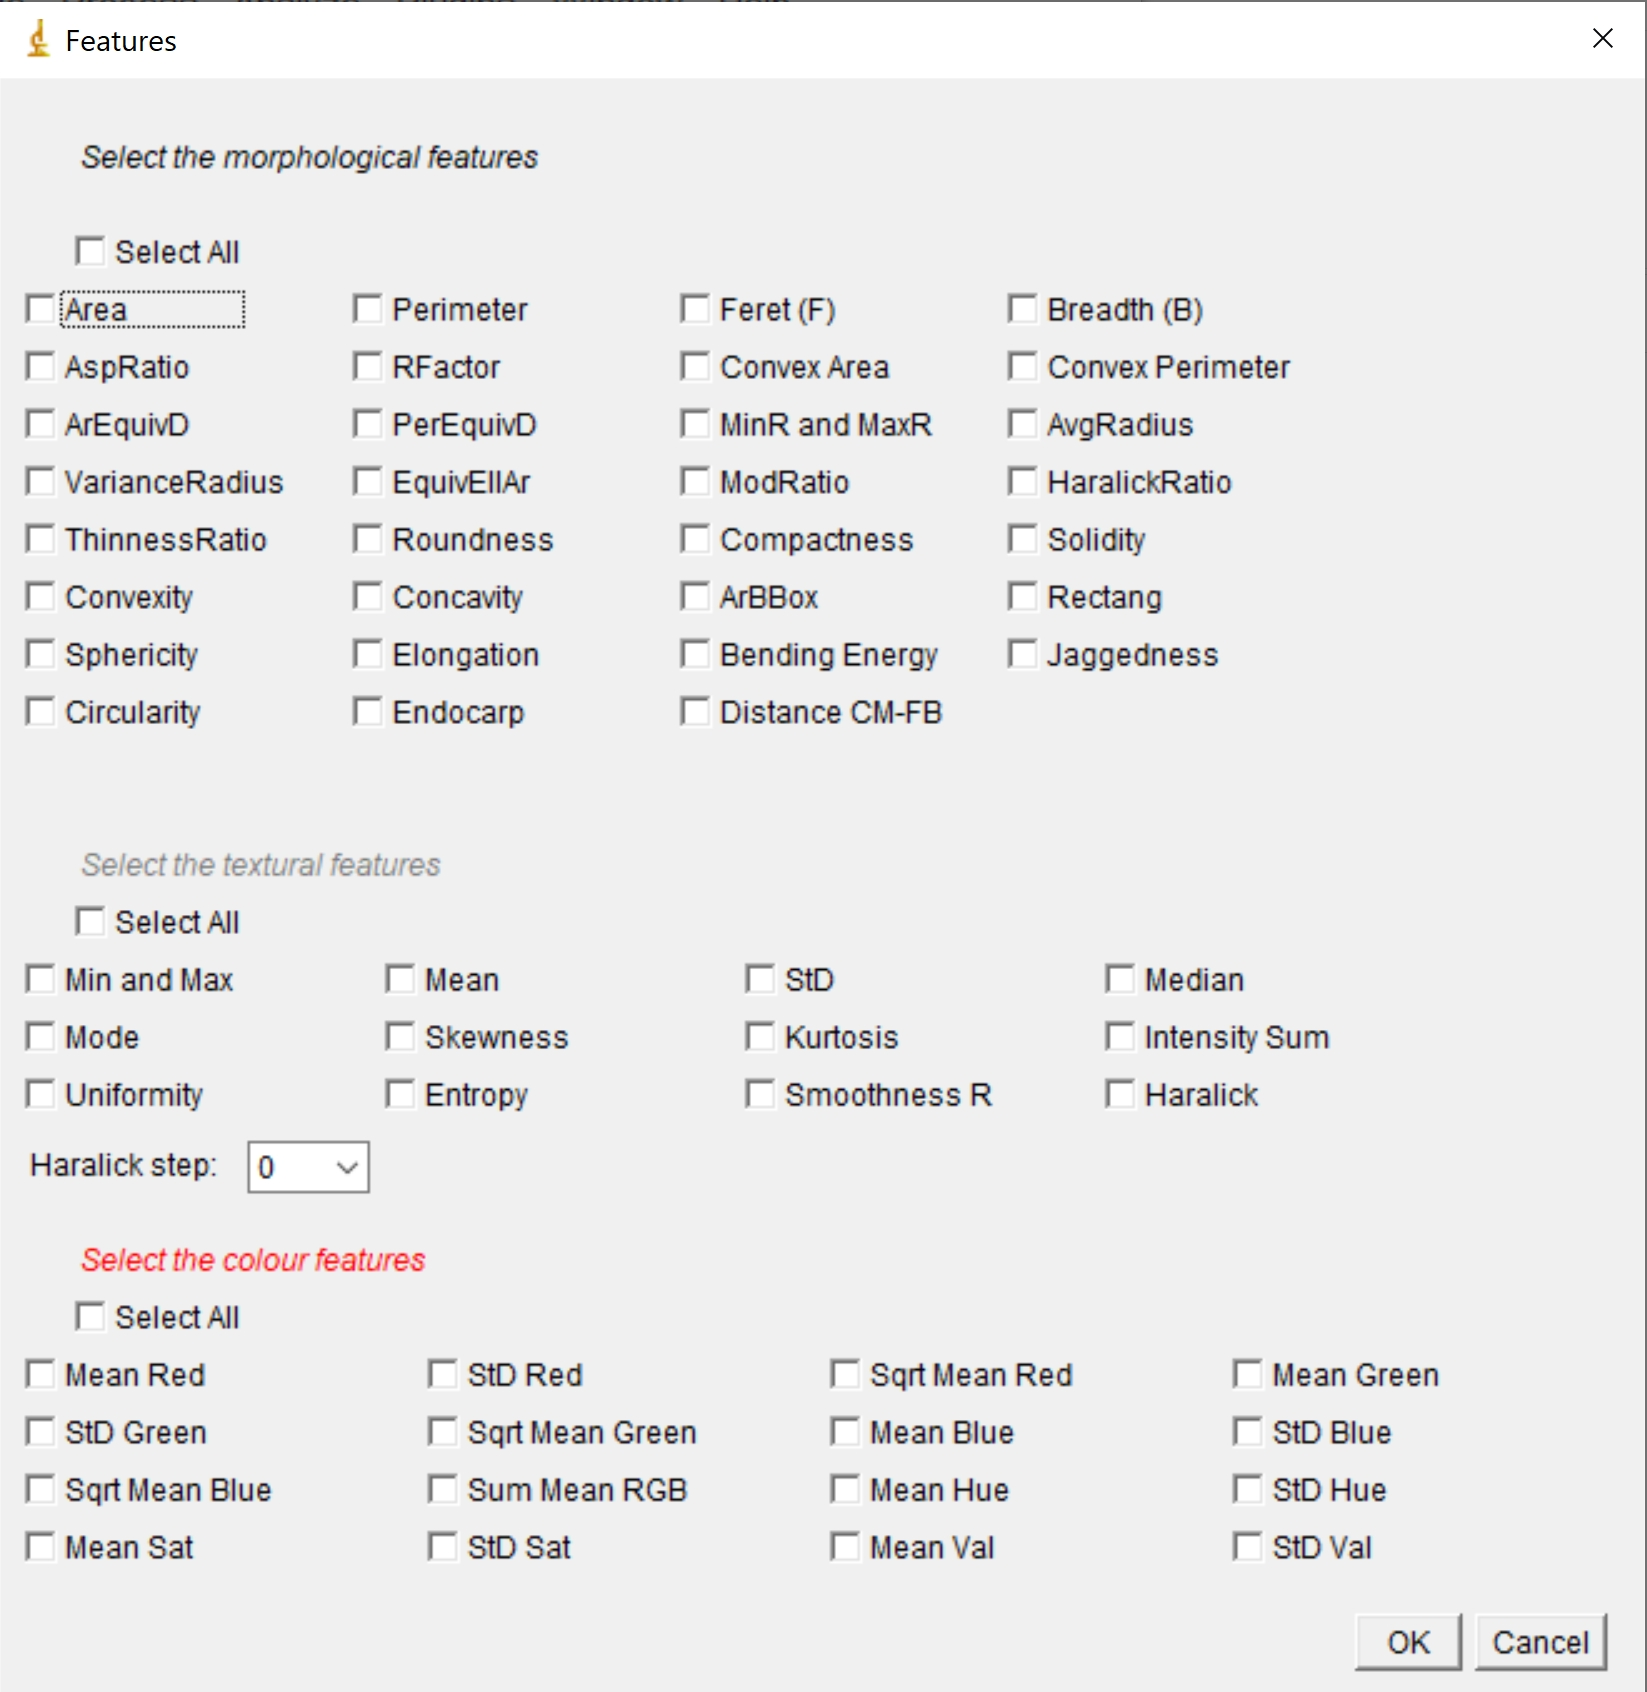
\includegraphics[height=0.35\textheight]{Features_selection.jpg}
	\caption{\label{fig:features_selection}Window for feature selection.}
\end{figure}

\emph{SeedsAnalyser} implements up to 64 features. In particular, 32 are morphological, 16 textural and 16 colour intensity values. It is crucial to notice that, among the texture features, Haralick's GLCM \cite{Haralick73}, which describes the pairwise arrangement of pixels with the same grey-level, was used in this study to extract information of local similarities. All of them permits their computation with the typical four different degrees: 0\degree, 45\degree, 90\degree, 135\degree. More precisely, we extracted the following second-order statistics from GLCM: energy, contrast, correlation and homogeneity.
ImageJ already contains a plugin that works in a way similar to \emph{Seeds Analyser}, even though it only offers 18 features, and it does not have a multi-image workflow.
To sum up, after the initial preprocessing step, our plugin can detect each single seed present in the original RGB image from which the user can select the morphological, textural and colour features to extract. Table \ref{table:morph} and Table \ref{table:gray} present the implemented morphological and textural features, respectively, and their relative descriptions, while Table \ref{table:col} describes the computed features of the RGB and HSV colour spaces.

\begin{table*}[htbp]
	\caption{Morphological features from binary image}
	\centering 
	\footnotesize
	\scalebox{0.90}{
		\begin{tabular}{ l l } 
			\hline
			\textbf{Feature} & \textbf{Description} \\
			\hline
			\emph{Area} & Seed area (in pixels) \\
			\emph{Perimeter} & Length of the seed contour \\
			\emph{Feret} & Longest traceable diameter with two points of the seed's outline as endpoints, called Lenght\\
			\emph{Breath} & Length of longest traceable axis perpendicular to the Feret, also called Width\\
			\textit{AspRatio} & \textit{Feret}/\textit{Breadth}, also called eccentricity or rectangularity ratio\\
			\emph{ConvexArea} & Area of the convex polygon drawn between the external points of the region\\
			\emph{ConvexPerimeter} & Perimeter of the convex polygon \\
			\textit{RFactor} & Shape factor, defined as $CovenxArea/(Feret\times pi)$\\
			\textit{ArEquivD} & Diameter of the circle with equivalent area of the region, defined as $\sqrt{4/\pi \times Area}$  \\
			\textit{PerEquivD} & Diameter of the circle having the same perimeter of the region, $Area/\pi$ \\
			\textit{MinR} and \textit{MaxR} & Radii of the inscribed and the enclosing circles centred at the center of mass\\
			\textit{AvgRadius} & Average length of the radii calculated starting from the center of mass \\
			\textit{VarianceRadius} & Variance of radii \\ 
			\textit{EquivEllAr} & Area of the ellipse having \emph{Feret} and \emph{Breadth} as axes \\
			\textit{Modification Ratio} & Shape measure, defined as $(2 \times MinR)/Feret$ \\
			\textit{Haralick Ratio} & Ratio between the average and the standard deviation of the radii \\
			\textit{ThinnessR} & Thinness Ratio, also called shape, given by $ Perimeter^2 / Area $ \\
			\textit{Roundness} & Measure of roundness, defined as $4 \times Area/(\pi \times Feret^2)$ \\
			\textit{Compactness} & Measure of compactness, expressed by $\sqrt{4/\pi \times Area/Feret}$  \\
			\textit{Solidity} & Measure of solidity, defined as $Area/ConvexArea$ \\
			\textit{Convexity} & Measure of convexity, also called roughness, defined as $ConvexPerimeter/Perimeter$ \\
			\textit{Concavity} & Measure of concavity, defined as $ConvexArea$ - $Area$\\
			\textit{ArBBox} & Area of the bounding box containing the region \\
			\textit{Rectangularity} & Also called extent, defined as $Area / ArBBox$ \\
			\textit{Sphericity} & Also called radius ratio, expressed by $MinR/MaxR$ \\
			\textit{Elongation} & Inverse of the circularity, defined as $Perim^2 / (4 \times \pi \times Area) $\\
			\textit{Bending Energy} & Defined as the sum of the squared curvature along the entire contour \\
			\textit{Jaggedness} & Measure representing if a seed is "serrated", defined as $(2\times \sqrt{\pi\times Area})/Perimeter$ \\
			\textit{Circularity} & Also called shape factor, obtained by $2\times \pi \times Area/Perimeter^2$ \\
			\textit{Endocarp} & Number of pixels forming the seed endocarp\\
			\textit{FBtoCM} & Distance between the intersection coordinates of seed length and width and center of mass \\
			\hline
	\end{tabular}}
	\label{table:morph}
\end{table*}

\begin{table*}[htbp]
	\caption{Texture features from grayscale image}
	\centering 
	\footnotesize
	\scalebox{0.95}{
		\begin{tabular}{ l l } 
			\hline
			\textbf{Feature} & \textbf{Description} \\
			\hline
			\textit{Min} and \textit{Max} & Minimum and maximum gray value in the region \\
			\textit{Mean} & Average gray value in the region\\
			\textit{StD} & Intensity standard deviation as contrast measure \\
			\textit{Median} & Median of the gray values \\
			\textit{Mode}  & Mode of the gray values \\
			\textit{Skewness} & Measure of the symmetry of the graylevel histogram around the average value \\
			\textit{Kurtosis} & Measure of the "tailedness" of the graylevel histogram \\
			\textit{Intensity Sum} & Sum of the gray values of the region \\
			\textit{Uniformity} & Maximum when all the gray levels in the histogram are equal \\
			\textit{Entropy} & Measure of variability of grey level distribution \\
			\textit{Smoothness R }& Measure of smoothness \\ 
			\textit{Haralick} & GLCM's computed second-order statistics (Energy, Contrast, Correlation, Homogeneity) \\
			\hline
	\end{tabular}}
	\label{table:gray}
\end{table*}

\begin{table}[htbp]
	\caption{Color features from RGB and HSV color spaces}
	\centering 
	\footnotesize
	\begin{tabular}{ l l } 
		\hline
		\textbf{Feature} & \textbf{Description} \\
		\hline
		\textit{Mean Red (MR) }& Average of Red channel values \\
		\textit{StD Red} & Standard deviation of Red channel values \\
		\textit{SqrtMean Red} & Square root of the mean value for Red channel  \\
		\textit{Mean Green (MG)} & Average of Green channel values \\
		\textit{StD Green} & Standard deviation of Green channel values \\
		\textit{SqrtMean Green} & Square root of the mean value for Green channel \\
		\textit{Mean Blue (MB)} & Average of Blue channel values \\
		\textit{StD Blue} & Standard deviation of Blue channel values \\
		\textit{SqrtMean Blue} & Square root of the mean value for Blue channel \\
		\textit{Mean RGB} & \( \frac{MR + MG + MB}{3} \)\  \\ 
		\textit{Mean Hue} & Average tone of Hue channel \\
		\textit{StD Hue} & Standard deviation of Hue channel values \\			
		\textit{Mean Sat} & Average tone of Saturation channel \\
		\textit{StD Sat} & Standard deviation of Saturation channel values \\
		\textit{Mean Val} & Average tone of Value channel \\
		\textit{StD Val} & Standard deviation of Value channel values \\
		\hline
	\end{tabular}
	\label{table:col}
\end{table}

\subsection{A plugin for feature classification}
\label{feature_classifier}
Up to now, we have obtained the features for each seed from \emph{SeedsAnalyser} \ref{seeds_analyser}, and they can now be fed to the classification plugin, called \emph{SeedsClassifier}.
It offers four different classifiers, namely kNN, Naive Bayes, Random Forest and SVM. Weka \cite{Weka} includes all of them; therefore, they can be imported individually from their respective packages. All classifiers belong to their java class, where they implement the Classifier interface responsible for defining and realising the classification procedure.
At the plugin's start, the user can choose whether to load an existing model or start a new training phase on new data. If the user chooses to proceed from scratch, i.e. also with the training phase, the user will be asked to enter the ARFF file's name with the training dataset. For practical reasons, this file must be located in the main folder of the framework. The predictions will be displayed in a window called Predictions.
As we mentioned earlier, \emph{SeedsClassifier} plugin allows for the use of four classification algorithms. We now briefly describe how they operate and differ from each other.
In general, Naive Bayes classifiers are probabilistic models that use Bayes' theorem with strict independence assumptions between the features. 
%
KNN uses the \textit{k} closest training samples in the dataset as input and then uses a neighbour voting strategy to rank and classify new objects. Generally speaking, the larger k is, the more the noise associated with classification is reduced, but class recognition becomes more difficult. 
%
The Support Vector Machine (SVM) is a non-probabilistic binary linear classifier that categorises objects by mapping examples to points in space to maximise the width of the distance between categories. 
%
Finally, Random Forest is made up of many individual decision trees that work together to form an ensemble. Each tree predicts a class, and the class with the most votes is the model prediction. However, there is a need for each tree not to correlate with the others. This would jeopardise the classifier's final decision. In this way, the trees protect each other from their errors.
%
Given our feature spaces' abundance and diversity, we choose these classifiers to ensure classification accuracy, flexibility, and data adaptation.